\chapter{\protect\hyperlink{:}{光学}}
\addtocontents{toc}{\protect\hypertarget{:}{}}


光学是研究光的产生、传播、接收以及光与物质相互作用的学科。从历史上看，光学经历了从几何光学到波动光学再到量子光学的发展过程。本章主要讨论波动光学的核心内容。


\section{\protect\hyperlink{:}{几何光学}}
\addtocontents{toc}{\protect\hypertarget{:}{}}

\subsection{\protect\hyperlink{:}{几何光学的基本定律}}
\addtocontents{toc}{\protect\hypertarget{:}{}}

当光的波长远小于所涉及的尺度时，可以用\textbf{光线}模型来描述光的传播——这就是几何光学。

\subsubsection{\protect\hyperlink{:}{直线传播定律}}
\addtocontents{toc}{\protect\hypertarget{:}{}}

在均匀介质中，光沿直线传播。

\subsubsection{\protect\hyperlink{:}{反射定律与折射定律}}
\addtocontents{toc}{\protect\hypertarget{:}{}}

\begin{theorem}[反射定律]
    入射光线、反射光线和界面法线在同一平面内，反射角等于入射角
    \begin{equation}
        \theta_r = \theta_i
    \end{equation}
\end{theorem}

\begin{theorem}[折射定律（斯涅尔定律）]
    入射光线、折射光线和界面法线在同一平面内，且
    \begin{equation}
        n_1\sin\theta_1 = n_2\sin\theta_2
    \end{equation}
    其中 $n_1$、$n_2$ 分别是两种介质的折射率，$\theta_1$、$\theta_2$ 分别是入射角和折射角。
\end{theorem}

\subsection{\protect\hyperlink{:}{薄透镜}}
\addtocontents{toc}{\protect\hypertarget{:}{}}

透镜是光学系统中最基本的元件。

\begin{definition}[薄透镜公式]
    对于薄透镜，物距 $s$、像距 $s'$ 和焦距 $f$ 之间的关系为
    \begin{equation}
        \frac{1}{s} + \frac{1}{s'} = \frac{1}{f}
    \end{equation}
    符号约定：实物 $s > 0$，虚物 $s < 0$；实像 $s' > 0$，虚像 $s' < 0$；凸透镜 $f > 0$，凹透镜 $f < 0$。
\end{definition}

横向放大率定义为
\begin{equation}
    M = \frac{h'}{h} = -\frac{s'}{s}
\end{equation}

$|M| > 1$ 表示放大，$|M| < 1$ 表示缩小；$M < 0$ 表示倒像，$M > 0$ 表示正像。


\section{\protect\hyperlink{:}{光的干涉}}
\addtocontents{toc}{\protect\hypertarget{:}{}}

\subsection{\protect\hyperlink{:}{光的相干性}}
\addtocontents{toc}{\protect\hypertarget{:}{}}

两列光波能够产生稳定的干涉图样，需要满足三个条件：
\begin{enumerate}
    \item 频率相同
    \item 振动方向相同（或有平行分量）
    \item 相位差恒定
\end{enumerate}

满足这三个条件的光称为\textbf{相干光}。由于普通光源发出的光是大量独立原子发出的波列，相位随机变化，因此通常需要将同一光源发出的光分成两束，再让它们相遇——这就是获得相干光的两种方法：\textbf{分波前法}和\textbf{分振幅法}。

\subsection{\protect\hyperlink{:}{杨氏双缝干涉}}
\addtocontents{toc}{\protect\hypertarget{:}{}}

杨氏双缝干涉是分波前法的经典实验，它首次证明了光的波动性。

\begin{figure}[htbp]
    \centering
    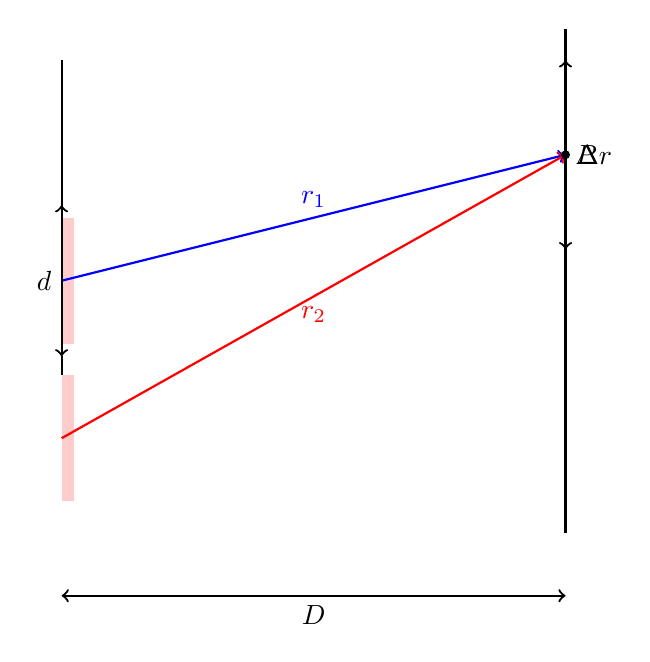
\begin{tikzpicture}[scale=0.8]
        \fill[red!20] (0,-1) rectangle (0.2,1);
        \fill[red!20] (0,-3.5) rectangle (0.2,-1.5);
        \draw[thick] (0,-1.2) -- (0,-1.5);
        \draw[thick] (0,1) -- (0,3.5);
        \draw[->,thick,blue] (0,0) -- (8,2) node[midway,above]{$r_1$};
        \draw[->,thick,red] (0,-2.5) -- (8,2) node[midway,below]{$r_2$};
        \fill (8,2) circle (2pt) node[right]{$P$};
        \draw[<->,thick] (8,0.5) -- (8,3.5) node[midway,right]{$\Delta r$};
        \draw[<->,thick] (0,1.2) -- (0,-1.2) node[midway,left]{$d$};
        \draw[<->,thick] (0,-5) -- (8,-5) node[midway,below]{$D$};
        \draw[thick] (8,-4) -- (8,4);
    \end{tikzpicture}
    \caption{杨氏双缝干涉示意图}
    \label{fig:杨氏双缝}
\end{figure}

设双缝间距为 $d$，缝到屏幕的距离为 $D$（$D \gg d$），屏幕上 $P$ 点到中心的距离为 $y$。

\begin{theorem}[杨氏双缝干涉的光程差]
    两列波到达 $P$ 点的光程差为
    \begin{equation}
        \Delta r = r_2 - r_1 \approx d\sin\theta \approx \frac{dy}{D}
    \end{equation}
\end{theorem}

\begin{proof}
    由几何关系，$r_1 = \sqrt{D^2 + (y - d/2)^2}$，$r_2 = \sqrt{D^2 + (y + d/2)^2}$。当 $D \gg d$ 且 $D \gg y$ 时，利用近似 $\sqrt{1+x} \approx 1 + x/2$
    \begin{equation}
        r_2 - r_1 = \sqrt{D^2 + (y+d/2)^2} - \sqrt{D^2 + (y-d/2)^2} \approx \frac{(y+d/2)^2 - (y-d/2)^2}{2D} = \frac{dy}{D}
    \end{equation}
\end{proof}

干涉条件为
\begin{enumerate}
    \item 明纹：$\Delta r = k\lambda$（$k = 0, \pm1, \pm2, \ldots$），对应位置
    \begin{equation}
        y_k = k\frac{D\lambda}{d}
    \end{equation}
    \item 暗纹：$\Delta r = (k + \frac{1}{2})\lambda$，对应位置
    \begin{equation}
        y_k = \left(k + \frac{1}{2}\right)\frac{D\lambda}{d}
    \end{equation}
\end{enumerate}

\begin{definition}[条纹间距]
    相邻明纹（或暗纹）之间的间距为
    \begin{equation}
        \Delta y = \frac{D\lambda}{d}
    \end{equation}
\end{definition}

\begin{remark}
    条纹间距 $\Delta y$ 与波长 $\lambda$ 成正比，与缝间距 $d$ 成反比。白光照射时，中央明纹为白色，两侧出现彩色条纹（紫光在内侧，红光在外侧）。
\end{remark}

\subsection{\protect\hyperlink{:}{薄膜干涉}}
\addtocontents{toc}{\protect\hypertarget{:}{}}

薄膜干涉是分振幅法的典型应用。光在薄膜上下两个表面反射后分成两束相干光，由于经过不同的光程，相遇时发生干涉。

\subsubsection{\protect\hyperlink{:}{半波损失}}
\addtocontents{toc}{\protect\hypertarget{:}{}}

\begin{definition}[半波损失]
    光从光疏介质（折射率小）射向光密介质（折射率大）时，反射光的相位会发生 $\pi$ 的突变，相当于多走了 $\lambda/2$ 的光程差。这就是\textbf{半波损失}。
\end{definition}

半波损失的判据：光从折射率 $n_1$ 射向 $n_2$，当 $n_1 < n_2$ 时，反射光有半波损失；当 $n_1 > n_2$ 时，反射光没有半波损失。

\subsubsection{\protect\hyperlink{:}{等厚干涉}}
\addtocontents{toc}{\protect\hypertarget{:}{}}

当薄膜厚度不均匀时（如劈尖、牛顿环），干涉条纹反映了等厚度线。

\paragraph*{劈尖干涉}

\begin{definition}[劈尖干涉的光程差]
    设劈尖的折射率为 $n$，劈尖角为 $\theta$，在厚度 $h$ 处，两束反射光的光程差为
    \begin{equation}
        \Delta = 2nh + \frac{\lambda}{2}
    \end{equation}
    其中 $\lambda/2$ 是半波损失的贡献。
\end{definition}

明纹条件：$\Delta = k\lambda$；暗纹条件：$\Delta = (k + \frac{1}{2})\lambda$。

相邻明纹（或暗纹）对应的厚度差为 $\Delta h = \lambda/(2n)$，对应的水平间距为
\begin{equation}
    l = \frac{\lambda}{2n\theta}
\end{equation}

\paragraph*{牛顿环}

\begin{definition}[牛顿环]
    在一个平凸透镜和一个平面玻璃之间形成一个空气劈尖。干涉条纹是以接触点为中心的同心圆环。第 $k$ 级暗环的半径为
    \begin{equation}
        r_k = \sqrt{kR\lambda}
    \end{equation}
    其中 $R$ 为透镜的曲率半径。
\end{definition}

\begin{remark}
    牛顿环的中心是暗点（因为接触点处 $h = 0$，光程差为 $\lambda/2$，满足暗纹条件）。利用牛顿环可以精确测量透镜的曲率半径。
\end{remark}

\subsubsection{\protect\hyperlink{:}{等倾干涉}}
\addtocontents{toc}{\protect\hypertarget{:}{}}

当薄膜厚度均匀时，干涉条纹反映了等入射角线。

\begin{definition}[等倾干涉的光程差]
    对于厚度为 $h$、折射率为 $n$ 的平行薄膜，反射光的光程差为
    \begin{equation}
        \Delta = 2nh\cos\theta_r + \frac{\lambda}{2}
    \end{equation}
    其中 $\theta_r$ 为折射角。
\end{definition}

等倾干涉的条纹是同心圆环，圆心在透镜的焦点上。条纹的级次从中心向外递减。

\subsection{\protect\hyperlink{:}{迈克耳孙干涉仪}}
\addtocontents{toc}{\protect\hypertarget{:}{}}

迈克耳孙干涉仪利用分振幅法产生两束相干光，通过移动反射镜改变光程差。其原理在光谱测量、精密长度测量等方面有重要应用。


\section{\protect\hyperlink{:}{光的衍射}}
\addtocontents{toc}{\protect\hypertarget{:}{}}

\subsection{\protect\hyperlink{:}{惠更斯-菲涅尔原理}}
\addtocontents{toc}{\protect\hypertarget{:}{}}

\begin{theorem}[惠更斯-菲涅尔原理]
    波前上的每一个面元都可以看作一个新的子波源，空间某点的光振动是所有子波在该点叠加的结果。
\end{theorem}

这一原理将惠更斯原理（定性描述波的传播）与叠加原理结合，为衍射现象提供了定量分析的基础。

\subsection{\protect\hyperlink{:}{单缝夫琅禾费衍射}}
\addtocontents{toc}{\protect\hypertarget{:}{}}

单缝衍射是衍射现象最基本的实例。设缝宽为 $a$，平行光垂直入射，在远处的屏幕上观察衍射图样。

\begin{theorem}[半波带法分析]
    将缝分成许多窄条，每个窄条发出子波。在衍射角 $\theta$ 方向上，缝的上下边缘之间的光程差为
    \begin{equation}
        \delta = a\sin\theta
    \end{equation}
    当 $\delta = k\lambda$（$k = \pm1, \pm2, \ldots$）时，整个缝被分成偶数个半波带，相邻半波带的贡献相互抵消——出现暗纹。
\end{theorem}

\begin{theorem}[单缝衍射的暗纹条件]
    \begin{equation}
        a\sin\theta = k\lambda, \qquad k = \pm1, \pm2, \ldots
    \end{equation}
\end{theorem}

\begin{definition}[中央明纹]
    中央明纹的角宽度为
    \begin{equation}
        \Delta\theta = 2\frac{\lambda}{a}
    \end{equation}
    缝越窄，中央明纹越宽——这是衍射的一个重要特征。
\end{definition}

\begin{remark}
    单缝衍射的强度分布为
    \begin{equation}
        I(\theta) = I_0 \left(\frac{\sin\beta}{\beta}\right)^2, \qquad \beta = \frac{\pi a\sin\theta}{\lambda}
    \end{equation}
    其中 $I_0$ 是中央极大的强度。中央明纹集中了绝大部分光能。
\end{remark}

\subsection{\protect\hyperlink{:}{圆孔衍射与光学仪器的分辨本领}}
\addtocontents{toc}{\protect\hypertarget{:}{}}

圆孔衍射的图样是一个中央亮斑（\textbf{艾里斑}）周围环绕着同心暗环和亮环。

第一暗环的角半径为
\begin{equation}
    \theta_1 = 1.22\frac{\lambda}{D}
\end{equation}

其中 $D$ 为圆孔直径。

\begin{theorem}[瑞利判据]
    两个点光源刚好能被分辨的条件是：一个像的中央明纹中心恰好落在另一个像的第一暗环上。此时两光源的角距离为
    \begin{equation}
        \theta_{\min} = 1.22\frac{\lambda}{D}
    \end{equation}
\end{theorem}

这表明：增大透镜直径 $D$ 或使用更短的波长 $\lambda$，可以提高光学仪器的分辨本领。

\subsection{\protect\hyperlink{:}{光栅衍射}}
\addtocontents{toc}{\protect\hypertarget{:}{}}

光栅是由大量等宽等距的平行狭缝组成的光学元件。设光栅常量为 $d$（相邻两缝的间距），缝宽为 $a$。

\begin{theorem}[光栅方程]
    主极大（明纹）的条件为
    \begin{equation}
        d\sin\theta = k\lambda, \qquad k = 0, \pm1, \pm2, \ldots
    \end{equation}
\end{theorem}

\begin{proof}
    相邻两缝在衍射角 $\theta$ 方向的光程差为 $d\sin\theta$。当光程差为波长的整数倍时，所有缝发出的光在该方向干涉相长，形成主极大。
\end{proof}

光栅衍射的特点：
\begin{enumerate}
    \item 主极大非常锐利，缝数 $N$ 越多，主极大越窄。
    \item 相邻主极大之间有 $N-1$ 个暗纹和 $N-2$ 个次极大。
    \item 缺级现象：当光栅方程和单缝暗纹条件同时满足时，该级主极大缺失，即当 $d/a$ 为整数时，第 $d/a$、$2d/a$、$\ldots$ 级主极大缺失。
\end{enumerate}

\begin{definition}[光栅的分辨本领]
    光栅的分辨本领为
    \begin{equation}
        R = \frac{\lambda}{\Delta\lambda} = kN
    \end{equation}
    其中 $k$ 为衍射级次，$N$ 为总缝数。缝数越多，分辨本领越高。
\end{definition}

\begin{remark}
    光栅衍射是单缝衍射和多缝干涉的综合效果。单缝衍射决定了主极大的包络线（强度分布），多缝干涉决定了主极大的位置和锐度。
\end{remark}


\section{\protect\hyperlink{:}{光的偏振}}
\addtocontents{toc}{\protect\hypertarget{:}{}}

\subsection{\protect\hyperlink{:}{自然光与偏振光}}
\addtocontents{toc}{\protect\hypertarget{:}{}}

\textbf{自然光}中电矢量的振动方向在垂直于传播方向的平面内随机分布，各个方向的振幅相等。

\textbf{偏振光}中电矢量的振动方向有确定性：
\begin{enumerate}
    \item \textbf{线偏振光}：电矢量沿一个固定方向振动。
    \item \textbf{圆偏振光}：电矢量的端点描绘出一个圆。
    \item \textbf{椭圆偏振光}：电矢量的端点描绘出一个椭圆。
\end{enumerate}

\subsection{\protect\hyperlink{:}{马吕斯定律}}
\addtocontents{toc}{\protect\hypertarget{:}{}}

\begin{theorem}[马吕斯定律]
    当线偏振光通过一个偏振片时，透射光的强度为
    \begin{equation}
        I = I_0\cos^2\theta
    \end{equation}
    其中 $I_0$ 是入射偏振光的强度，$\theta$ 是入射偏振方向与偏振片透振方向之间的夹角。
\end{theorem}

\begin{proof}
    线偏振光的电矢量可以分解为平行于透振方向和垂直于透振方向的两个分量。只有平行分量能通过偏振片，其振幅为 $E_0\cos\theta$。由于强度与振幅的平方成正比
    \begin{equation}
        I = (E_0\cos\theta)^2 = I_0\cos^2\theta
    \end{equation}
\end{proof}

\begin{remark}
    当 $\theta = 90°$ 时，$I = 0$——透振方向垂直的偏振片完全阻挡线偏振光。当自然光通过偏振片后，变成线偏振光，强度为原来的一半（$I = I_0/2$）。
\end{remark}

\subsection{\protect\hyperlink{:}{布儒斯特定律}}
\addtocontents{toc}{\protect\hypertarget{:}{}}

\begin{theorem}[布儒斯特定律]
    当光以特定角度（\textbf{布儒斯特角} $\theta_B$）入射到两种介质的界面时，反射光为完全偏振光。布儒斯特角满足
    \begin{equation}
        \tan\theta_B = \frac{n_2}{n_1}
    \end{equation}
    此时反射光线与折射光线相互垂直（$\theta_B + \theta_r = 90°$）。
\end{theorem}

\begin{proof}
    当入射角为布儒斯特角时，反射光和折射光垂直，即 $\theta_B + \theta_r = 90°$。由折射定律 $n_1\sin\theta_B = n_2\sin\theta_r$，代入 $\theta_r = 90° - \theta_B$
    \begin{equation}
        n_1\sin\theta_B = n_2\sin(90° - \theta_B) = n_2\cos\theta_B
    \end{equation}
    即 $\tan\theta_B = n_2/n_1$。
\end{proof}

\begin{remark}
    布儒斯特定律的一个重要应用是：利用偏振片可以消除反射光的眩光。例如，偏振太阳镜就是利用布儒斯特定律来减少水面或路面的反射眩光。
\end{remark}

\subsection{\protect\hyperlink{:}{双折射}}
\addtocontents{toc}{\protect\hypertarget{:}{}}

\begin{definition}[双折射]
    某些晶体（如方解石）具有\textbf{双折射}性质：一束光进入晶体后分成两束——寻常光（$o$ 光）和非常光（$e$ 光），它们都是线偏振光，且偏振方向相互垂直。
\end{definition}

\begin{definition}[光轴]
    晶体中存在一个特殊方向，光沿此方向传播时不发生双折射，这个方向称为\textbf{光轴}。
\end{definition}

\begin{definition}[波片]
    波片是利用双折射原理制成的光学元件。当光垂直入射到波片时，$o$ 光和 $e$ 光在晶体内传播速度不同，产生光程差。
    \begin{enumerate}
        \item \textbf{四分之一波片}：$o$ 光和 $e$ 光的光程差为 $\lambda/4$，可将线偏振光变为圆偏振光。
        \item \textbf{半波片}：$o$ 光和 $e$ 光的光程差为 $\lambda/2$，可将线偏振光的偏振方向旋转 $90°$。
    \end{enumerate}
\end{definition}

\begin{remark}
    偏振光的分析在光学中非常重要。通过组合偏振片和波片，可以实现各种偏振态的转换和检测。这在液晶显示（LCD）、光学通信、光弹性力学等领域有广泛应用。
\end{remark}
